\subsection{PHP}
\label{sec:php}
The main programming language chosen for the backend development of the application is PHP. This language has been chosen for several reasons, namely that we are familiar with it, it is well-documented and that it is open source.

\subsubsection{FuelPHP Framework}
\label{sec:fuelphp_framework}
\begin{quote}
FuelPHP is a simple, flexible, community driven PHP 5.3 web framework based on the best ideas of other frameworks with a fresh start\cite{FuelPHP}.
\end{quote}

FuelPHP\footnote{See \cite{FuelPHP} for more documentation} uses a HMVC\footnote{Hierarchical model-view-controller} pattern and comes with different tools for fast and flexible development of web applications. Past experience with the framework and the fact that it takes advantage of the object orientation of PHP has been the main reason for why it was chosen. Notable tools and packages that have been heavily used while developing the application are:

\begin{itemize}
\item Oil - a command line utility that can be used for development, such as code scaffolding and running tasks. 
\item Migration - a task that makes it easy to manage database design via. revisions.
\item Tasks - classes that can be run directly in the command line or set up as cron jobs.
\item SimpleAuth - a package containing an authentication driver
\end{itemize}

\subsubsection{Administration}
\label{sec:administration}
An administration panel has been created to provide management of the data without having to think of unauthorized use. It also provides a simple overview, as seen on figure \ref{fig:admin}, and CRUD for the files and can be expanded to provide even more information easily.

\begin{figure}[htbp]
   \centering
   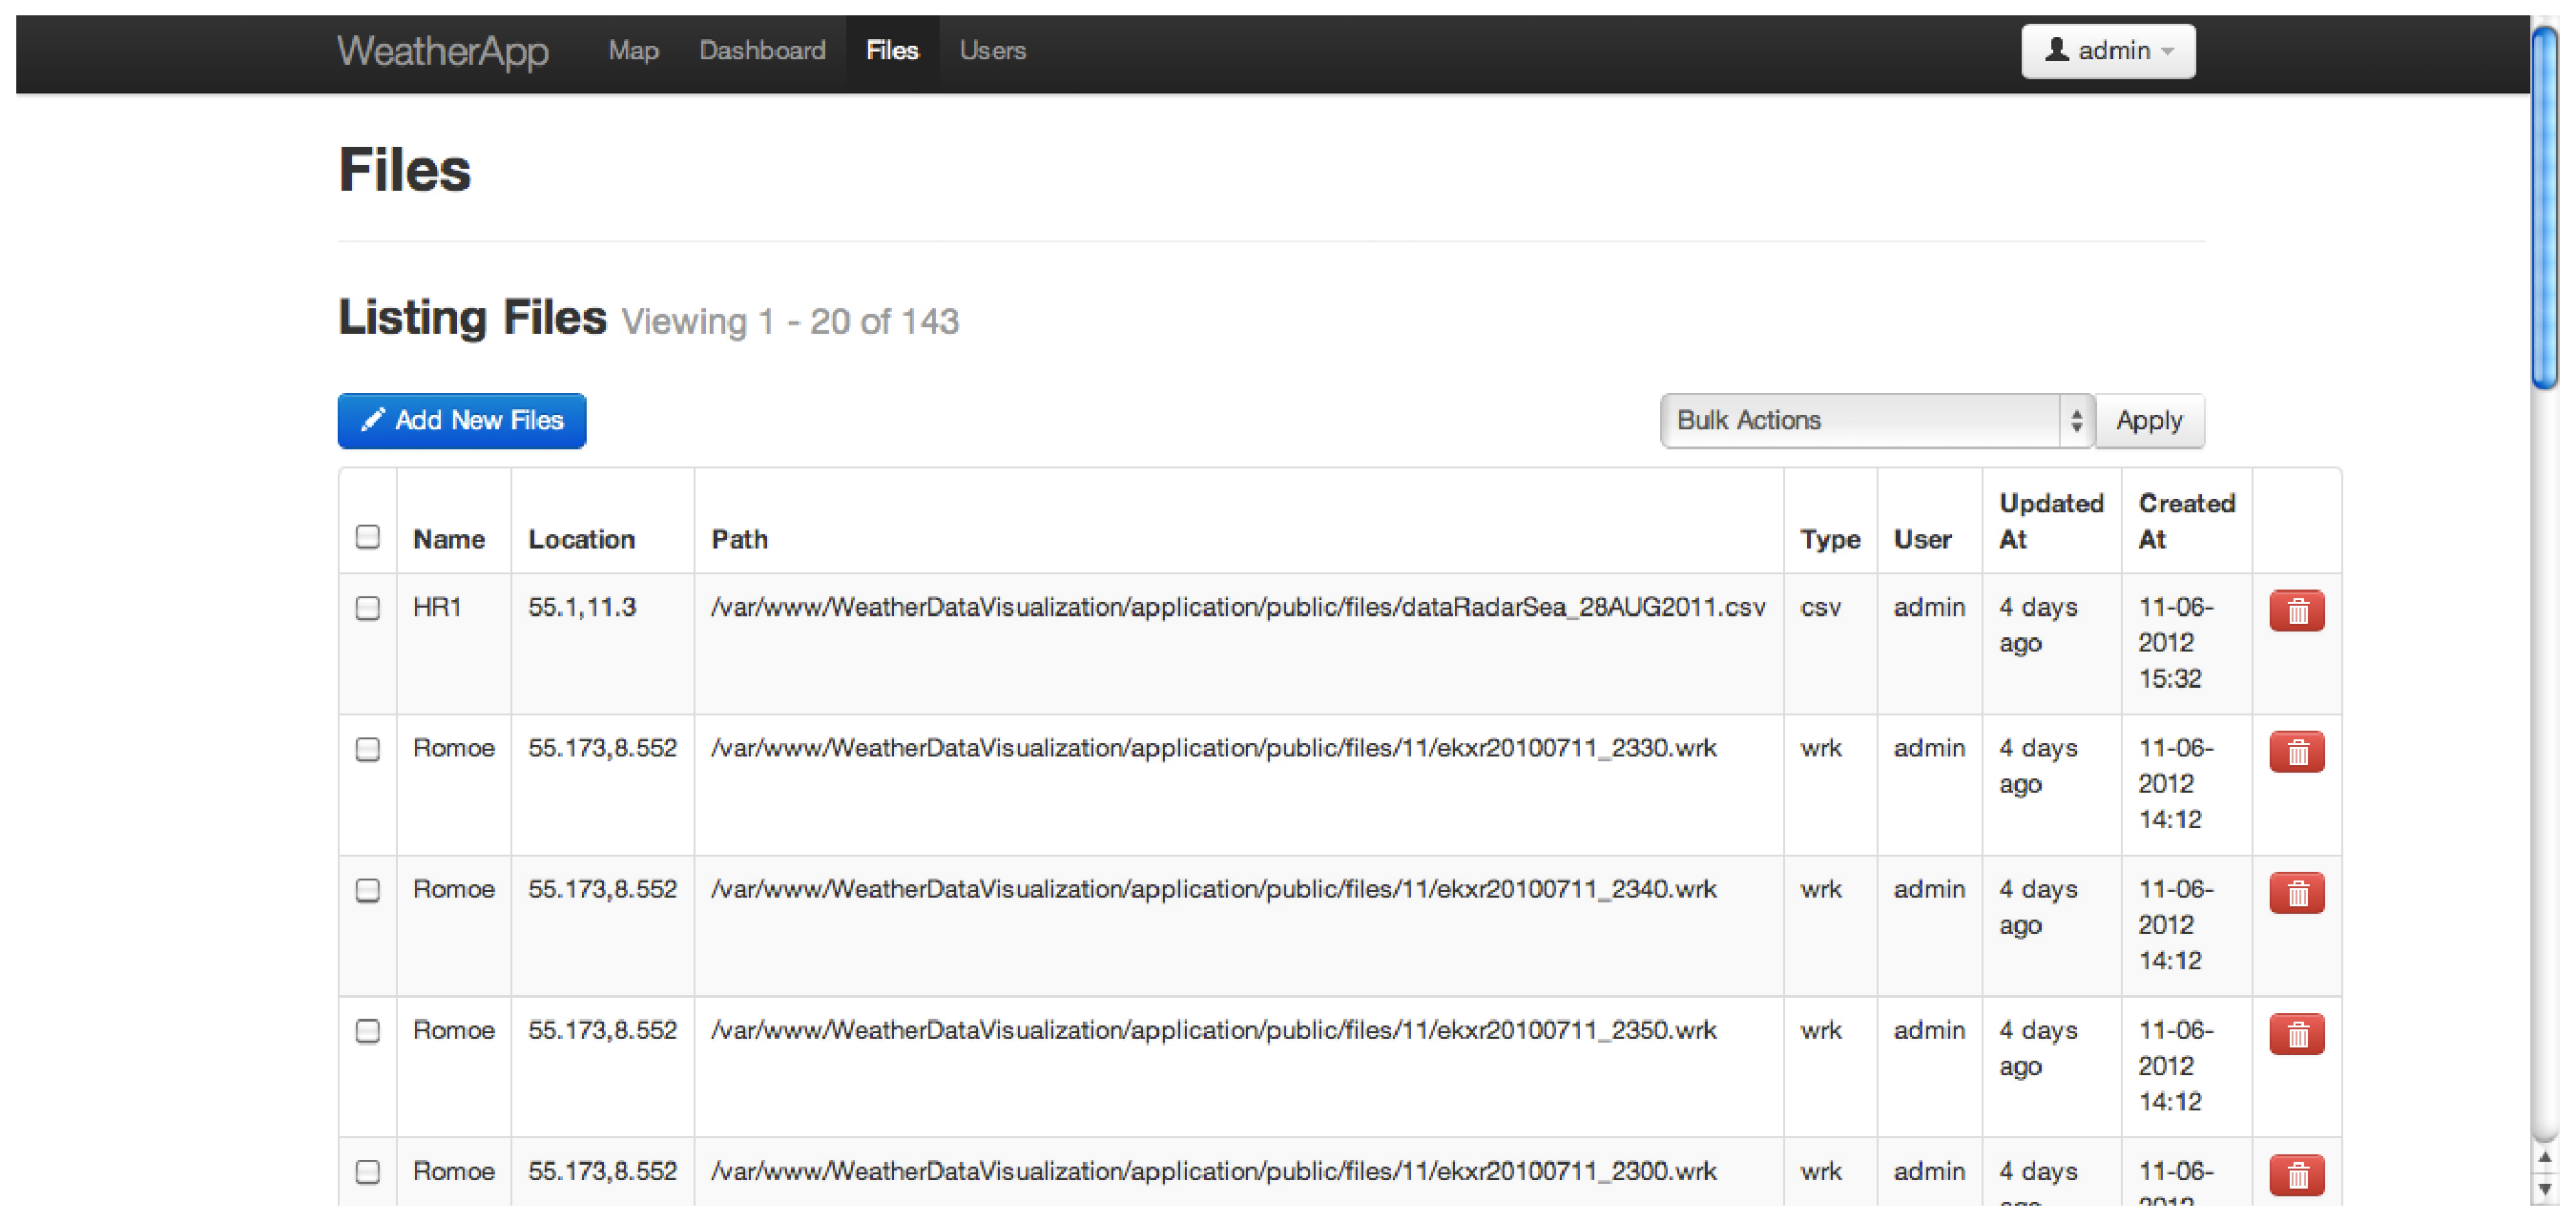
\includegraphics[width=.95\linewidth]{figure/adminCRUD.eps}
   \caption{Files overview}
   \label{fig:admin}
\end{figure}

\subsubsection{Tasks}
\label{sec:tasks}
When first uploading files in the administration, data was parsed in real time, which could lead to a time out by the server, if too many files were uploaded. To avoid this, a \textsf{Task} called \textsf{preparedata} was created to handle the parsing of the data, that is, running the data parser and inserting the data in the database. As \textsf{preparedata} is running, it will check whether there are any uploaded files that has not yet got their data parsed - if there are, these will be parsed. This check will be performed every 5 seconds, until the \textsf{preparedata} is stopped manually.
The main advantages of using a \textsf{Task} for this job are that it can handle a heavy amount of data without getting time out errors, it can be set up as a cron job, and it is possible to deploy it on another server than the application webserver.
In fact, \textsf{Tasks} are quite powerful tools as they can ultimately remove huge bottlenecks from the application webserver by running them on one or several other servers. E.g. files of type \textsf{csv} can be parsed on one server, while those of type \textsf{wrk} can be parsed on another, both independent of the application webserver.

\subsubsection{Timezones}
\label{sec:timezones}
When a user uploads a file in the administration, he must pick what timezone the data has been observed in as seen on figure \ref{fig:upload}. As the dataparser task handles the data for this file, the timezone will be converted to UTC - possible daylight saving time is detected and considered automatically. All data in the application will therefore be in UTC.

\begin{figure}[htbp]
   \centering
   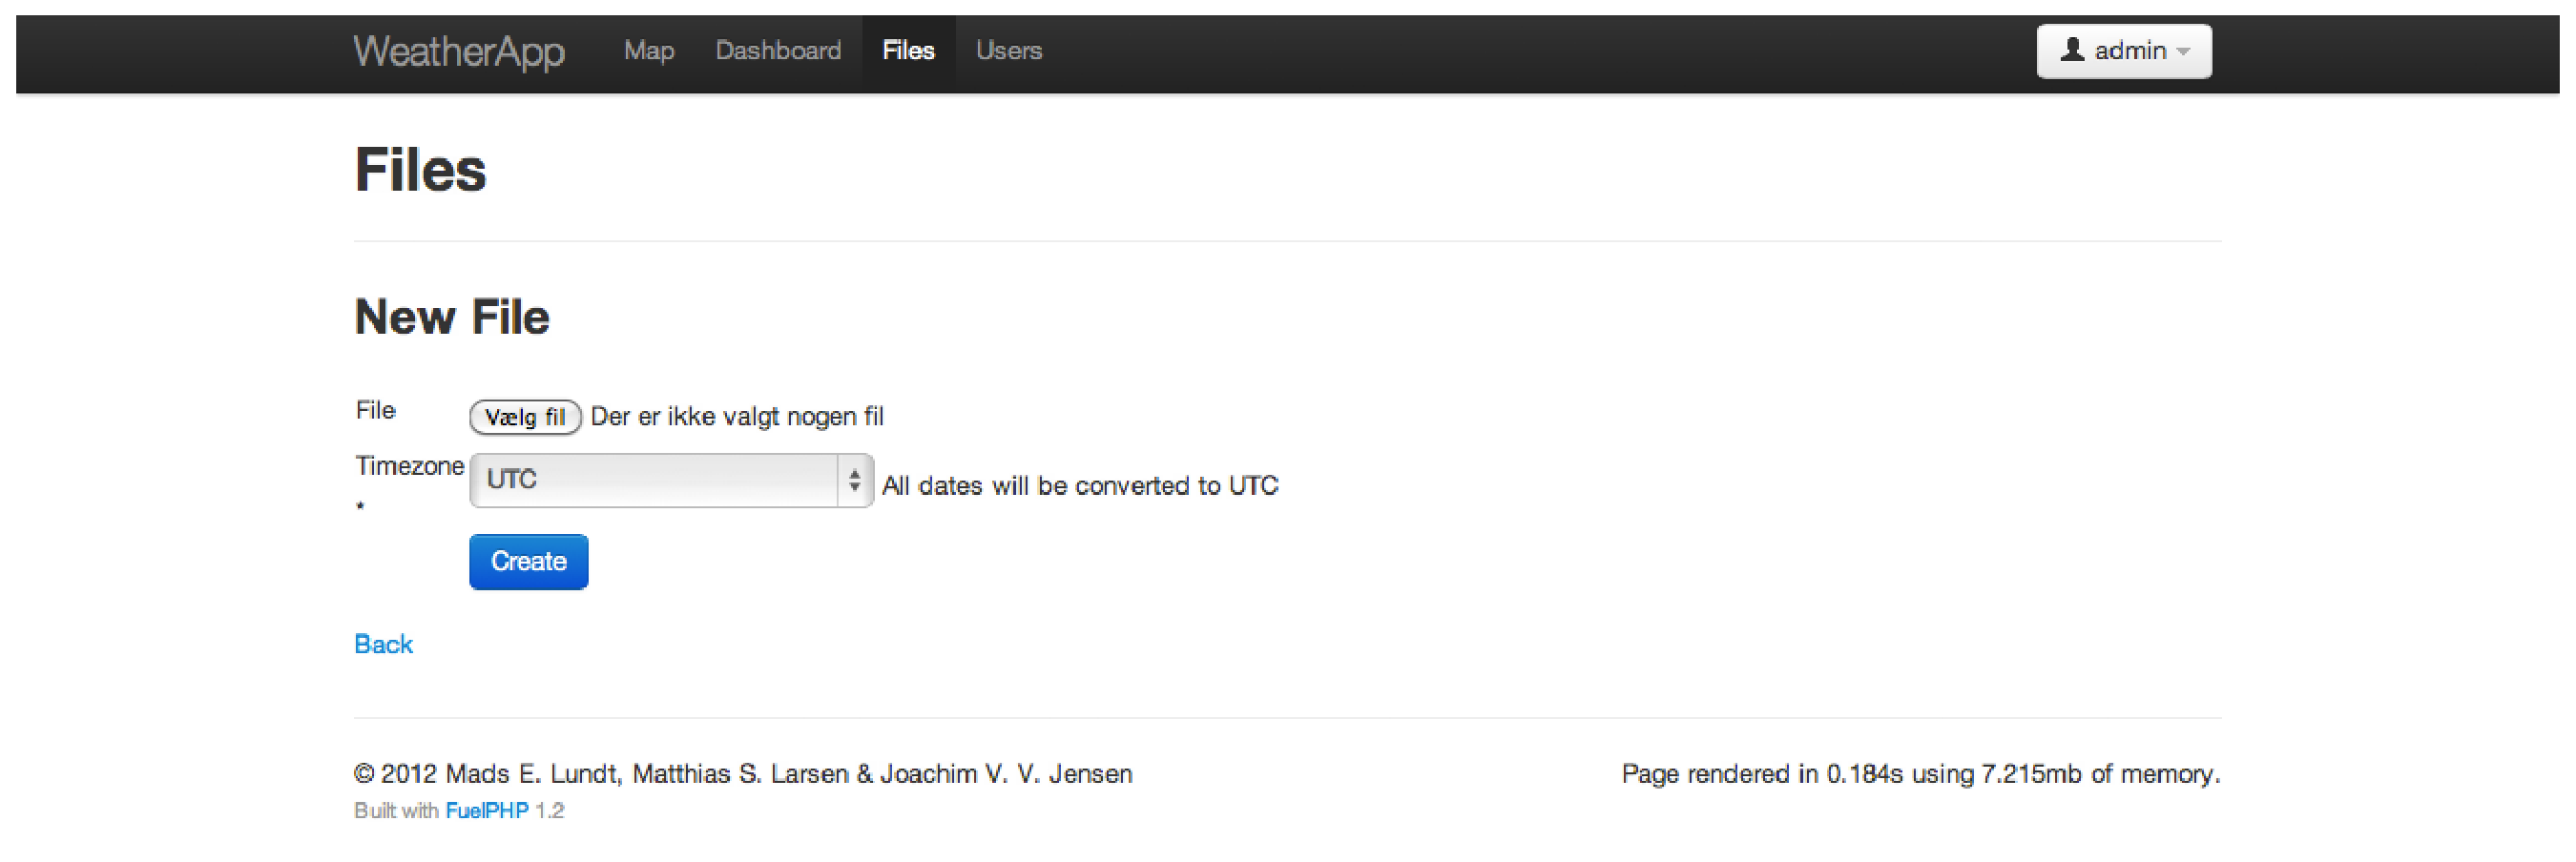
\includegraphics[width=.95\linewidth]{figure/uploadfiles.eps}
   \caption{Uploading files}
   \label{fig:upload}
\end{figure}